\chapter{Applicazioni future}
\label{cha:intro}
\vspace{5mm}

Uno degli aspetti principali che hanno portato al refactor di questo progetto è stata quella di renderlo più flessibile ed adattabile ad altri contesti e non solo legato al comune che ha commissionato l’applicativo. Un ulteriore passo in questa direzione è lo sviluppo di un altro applicativo che abbia le funzionalità di un orchestratore. Tale applicativo, anch'esso sviluppato mediante Nodejs sarà in grado di sfruttare a pieno l’alta configurabilità di ogni applicativo che comprende lo stack Alakai, eseguendo in modo automatizzato la configurazione e il deploy di tutti i servizi necessari. Per raggiungere tale scopo è necessario implementare alcuni accorgimenti. I punti che descriverò ora sono delle linee guida generali e non passaggi sequenziali verso un prodotto finito.\vspace{5mm}

Il primo tra questi è possedere un portale dove richiedere all’utente le configurazioni necessarie, come il nome dell’applicativo, se si desidera utilizzare o meno l’Estimote SDK oppure utilizzare il GPS, le Api key di Eventbrite e le chiavi degli store per la firma degli applicativi per IOS e per Android. Una volta ottenute queste informazioni è necessario costruire un manager che, una volta importata la configurazione, esegua un deploy della parte server in Nodejs, trasponga l’applicativo admin in React e lo inserisca all’interno di una directory prestabilita sul server in modo che possa essere servito staticamente e infine compili e firmi i due applicativi per Android e IOS. Le problematiche da risolvere per raggiungere un prodotto di questo tipo sono molteplici, ne discuterò solo alcune.\vspace{5mm}

E’ necessario possedere un ambiente in grado di ospitare un applicativo in Nodejs e servire mediante un proxyPass sia l’applicativo in React sia le Api sullo stesso dominio. Per fare questo è necessario che la macchina abbia installata una versione di Node Js superiore al 6 e aver installato e configurato Nginx o Apache in modo da implementare il proxyPass descritto sopra. Tali configurazioni sono di fatto uguali ad ogni istanza che si desidera allocare per cui una soluzione per gestire ed automatizzare il tutto è utilizzare un'immagine Docker. Docker permette di creare delle istanze, chiamate container, separate dal sistema operativo che le ospita.Tali istanze sono meno pesanti rispetto ad una macchina virtuale, questo grazie alla condivisione delle risorse del kernel tra i vari container. Oltre a ciò sono, grazie alla condivisione delle risorse a basso livello, molto veloci da avviare e da arrestare e questo rende Docker la tecnologia perfetta per questo genere di problematiche.
L’idea è quella di creare un immagine docker che contiene NodeJs e Nginx insieme alla sua configurazione ed iniettare all’interno di essa, al momento della creazione dell’istanza, il codice sorgente configurato mediante i dati inviati dall’utente.\vspace{5mm}

Per quanto riguarda invece la compilazione e la firma degli applicativi mobili è necessario configurare in modo particolare la macchina che eseguirà questo tipo di task. Di fatto bisogna che sia una versione di macOs visto che Apple non fornisce ad ora una versione di XCode per sistemi linux o Windows. Per quanto riguarda Android è necessario installare la command line interface del Gradle. A questo punto sarà necessario preparare uno script in bash che eseguirà una volta chiamato, tutte le procedure di compilazione e di firma degli applicativi. Tale procedura dovrà renderli disponibili al download inserendoli in una apposita directory dove un applicativo gli servirà e potranno essere scaricati e distribuiti attraverso gli store.\vspace{5mm}

Questi sono alcuni dei punti implementativi da svolgere per arrivare ad avere un prodotto con queste features. L’architettura progettuale risultante sarà simile a quella descritta in figura\vspace{5mm}

\begin{figure}[h]
\centering
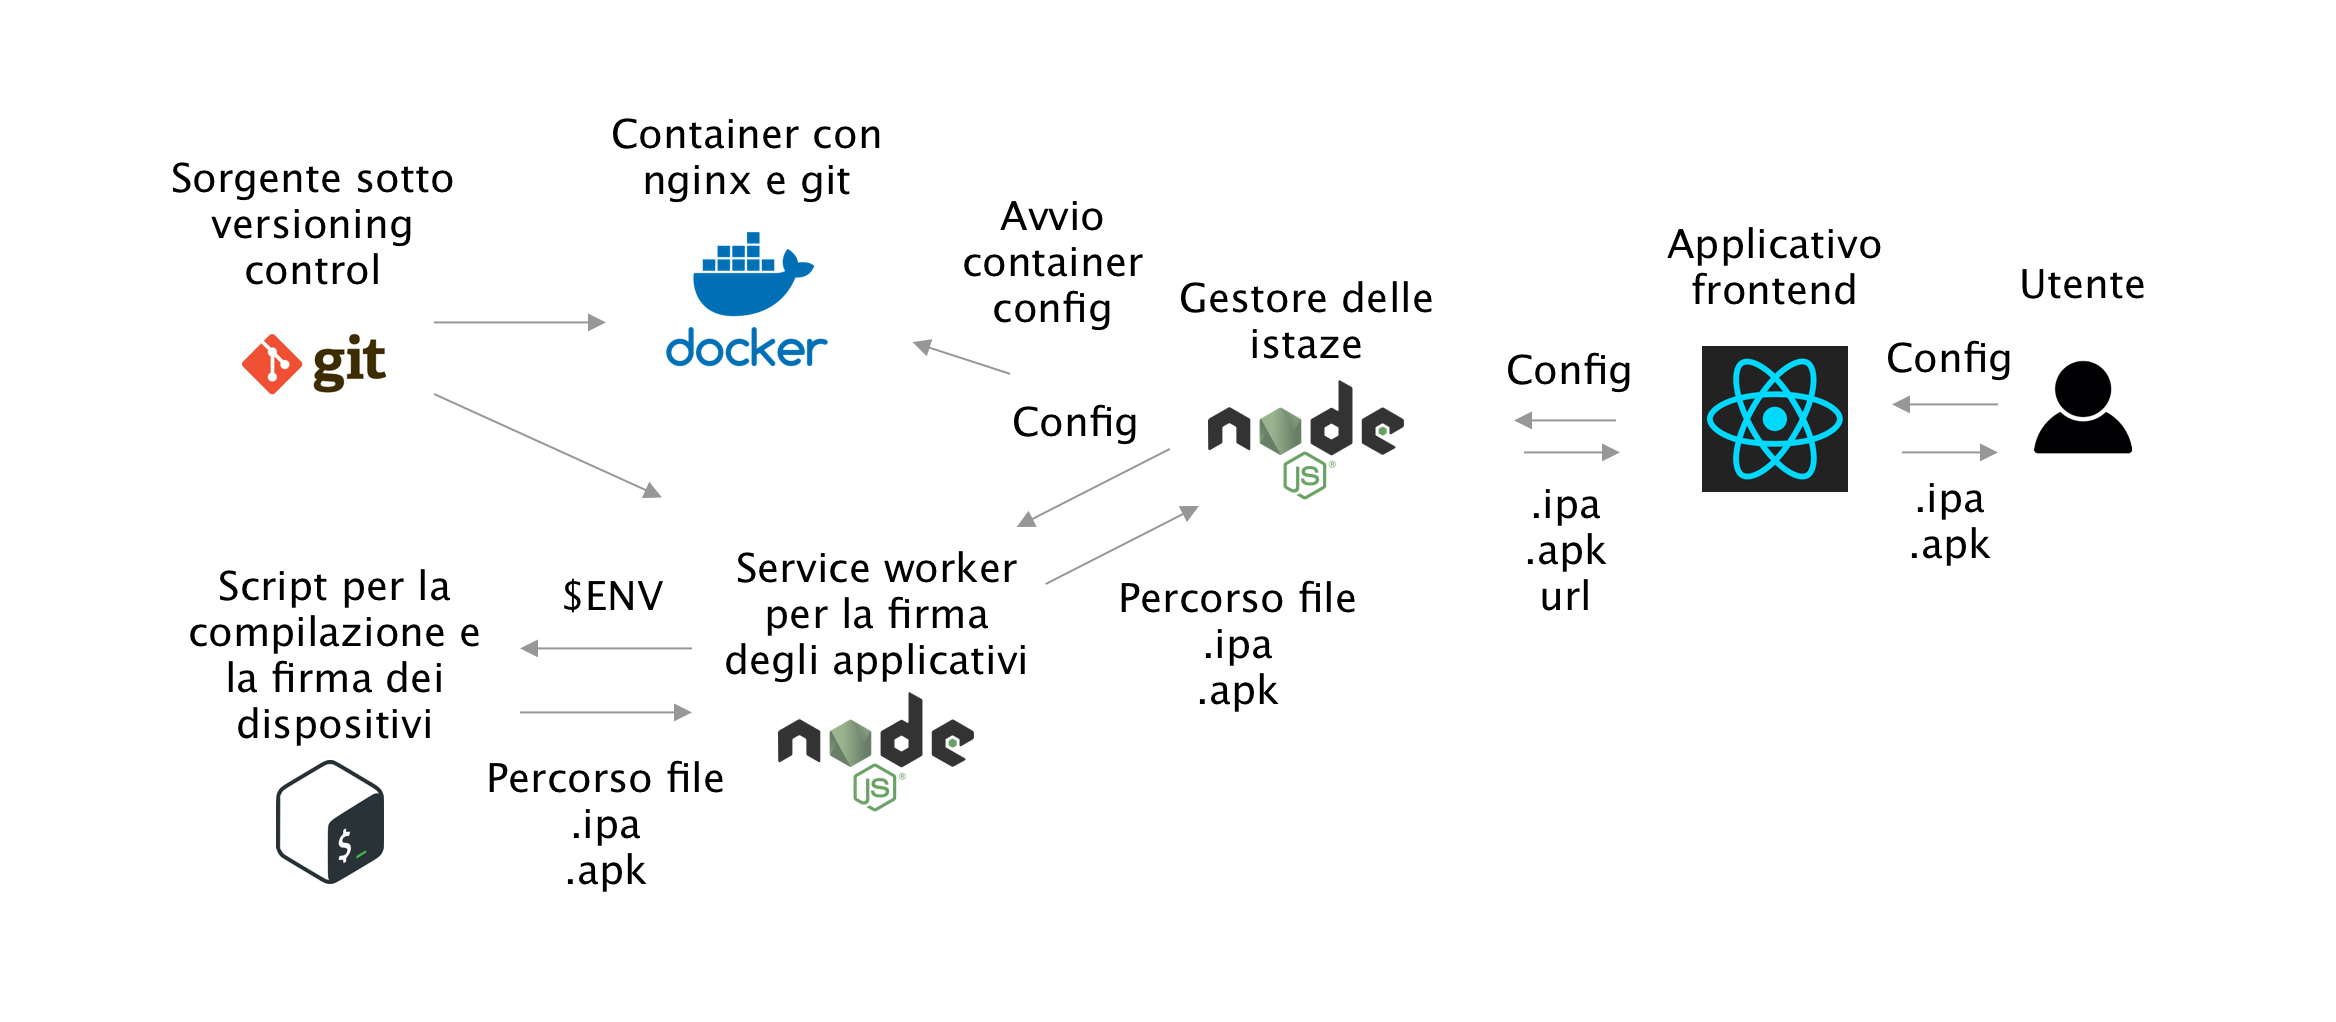
\includegraphics[width=1\textwidth]{images/schemaIstanzeAlakai.png}
\caption{Schema del funzionamento della possibile futura del Control Manager di istanze di Open Air Museum}
\end{figure}

Come si può notare vi sarà un service worker sviluppato in node che controllerà l’esecuzione dello script bash iniettando tutte le variabili di environment come i percorsi ai certificati ,precedentemente caricati, indispensabili per la procedura di compilazione e di firma.\vspace{5mm}

\section{Esecuzione di processi in Nodejs}
\vspace{5mm}Per rendere possibile questo tipo di prodotto è necessario che l'applicativo in Javascript sia in grado di pilotare uno script bash. Per fare questo è possibile utilizzare il modulo ChildProcess\cite{ChildProcess} che espone una serie di metodi di esecuzione possibili. Tra quelle disponibili vi è l'esecuzione attraverso spawn che esegue lo script indicato all'interno di un processo generato come figlio di quello principale. Il controllo dello stato di questo processo avviene attraverso gli stream di output che questo processo utilizza come standard output. Per esempio nel caso di un programma in c++ che stampa a console la somma tra due numeri passati come parametri, lo standard output è descritto dalla libreria iostream il quale compito è fare da ponte tra l'esecuzione del processo e la shell che lo sta eseguendo. Node.js tramite l'interfaccia a stream è in grado di agganciarsi a questo output e ridirigerlo in modo asincrono a Javascript che sarà in grado di mettere in coda l'esecuzione della funzione associata all'evento 'data' e di usufruire in modo asincrono e non bloccante dell'output del programma in c++ sopracitato.

\begin{figure}[h]
\centering
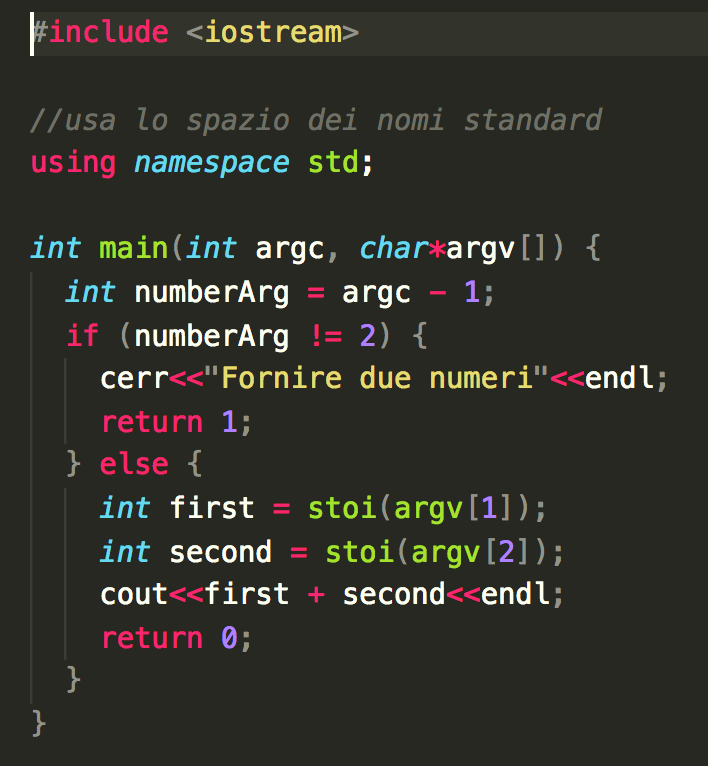
\includegraphics[width=0.4\textwidth]{images/cppCode.png}
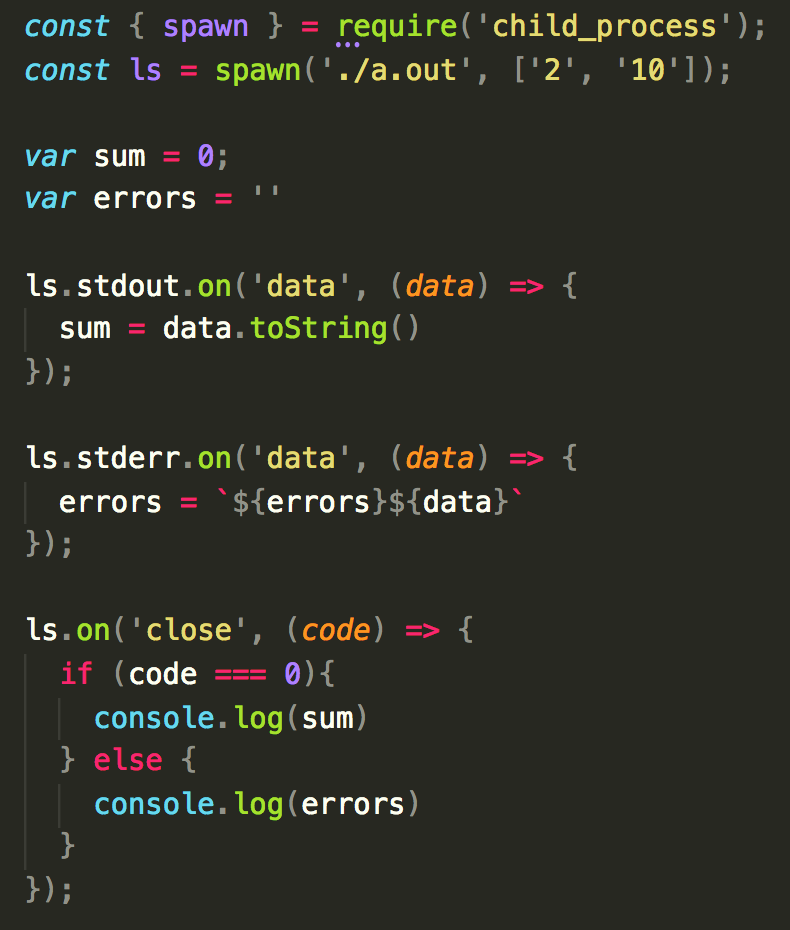
\includegraphics[width=0.4\textwidth]{images/jsCode.png}
\caption{Esempio di esecuzione codice c++ da Javascript}
\end{figure}

\vspace{5mm}Come si può vedere dalla figura 4.2 l'immagine a destra è il codice in c++ che verifica l'esistenza di soli due argomenti e nel caso gli converte in interi ed esegue la somma stampandola mediante cout che non fa altro che convertire tale valore in stringa inviandolo poi allo standard output. Passando all'immagine di destra si può vedere come mediante il modulo child-process e il metodo spawn si crea un processo utilizzando il risultato della compilazione del precedente codice c++ passando come parametri i due numeri che si desiderano sommare. Successivamente Javascript, in modo asincrono, si mette in ascolto dello standard output del processo catturandone i valori. Una volta che il processo ha completato l'esecuzione viene lanciato l'evento 'close' passando come parametro nel callback il codice di uscita del processo. Nel caso in cui esso sia uguale a zero il processo è stato eseguito correttamente e si può mostrare i risultati raccolti dall'esecuzione, altrimenti si mostrano gli errori. Da notare come nel caso in cui i numeri passati al processo in c++ sono diversi da sue il return del main torna 1 e sta ad indicare che vi è stato un errore e quindi vengono mostrati invece tutti gli output raccolti da stderr che è lo standard output per gli errori.

\vspace{5mm}Come si può intuire questa soluzione non è molto scalabile dato che utilizzare lo standard output per ricevere il risultato di un operazione potrebbe essere difficile nel caso di logiche più complesse. La soluzione potrebbe essere quella di utilizzate un ponte di comunicazione tra processi come Redis Pub/Sub \cite{PubSubRedis} in modo da poter comunicare attivamente in modo asincrono da entrambi i lati. Non descriverò nel dettaglio l'implementazione di questa soluzione perchè esula dallo scopo della tesi, ma offre un punto di partenza per lo sviluppo di una libreria per NodeJs per la compilazione automatica di applicativi nativi (ios e android).









